\newpage
\begin{center}
  \textbf{\large 3. Разработка алгоритма пост-коррекции с языковой моделью}
\end{center}
\refstepcounter{chapter}
\addcontentsline{toc}{chapter}{3. Разработка алгоритма пост-коррекции с языковой моделью}

Начнём здесь сначала с определения пост-коррекции.
Это подход, при котором мы корректируем расшифровки системы распознавания речи.
Наша основная идея в обучение языковой модели на русском языке для исправления ошибок.
Как мы обсуждали ранее, в основном алгориты, завязанные на LM полагаются на скрытое представление ASR модели или же на её проекцию в скрытое представление LM.
В противовес эту, мы действуем не в скрытом пространстве аудио модели, а в текстовом представление информации.
То есть мы будем сначала транскрибировать аудио в текст и только потом его править.
Таким образом мы решим проблему независимости ASR-LM пары, так как не нужно будет обучать языковую модель для понимания токенов ASR.
Недостатком такого подхода можно назвать то, что наши языковые модели будет необходимо обучать для нескольких языков в случае использования мультиязычной модели распознавания речи.
Допустим, мы возьмём Whisper, который может распознавать слова на разных языках.
Однако данная тема находится за пределами данной работы.

\section{Генерация датасета}
Теперь необходимо создать датасет для обучения.
Для этого возьмём и сгенерируем 5 гипотез с помощью BeamSearch алгоритма\cite{chen2023hyporadise}.
Затем мы подадим все 5 гипотез в нашу модель и попросим сгенерировать исправленную последовательность.

Почему подавать 5 гипотез в модель? Что мы можем взять из гипотез?
Почему просто не реранжировать гипотезы?
Давайте проанализируем полученные данные.

На рисунке~\ref{fig:dist} представлены графики распределение токенов.
На первом из них изображено распределение токенов из Ground Truth (GT) в гипотезах.
В данном случае мы считаем вероятность найти токен из «правильной» транскрипции в наших гипотезах.
Как можно заметить, вероятности достаточно близки.
На втором графике показано вероятность найти в гипотезе $i$ токена, которого не было в гипотезах до этого.
То есть, в столбце для гипотезы 3 показана вероятность найти токен, которого не было до этого в гипотезах 1-2, но который есть в «правильной» транскрипции.
Хорошо показано, что достаточно малый процент токенов остаётся даже до второй, где вероятность от 0.07 до 0.025.
Третий график показывает, какой процент токенов из Ground Truth входит в наши 5 гипотез, а какой нет.
Можно увидеть, что у RuLibriSpeech и OpenSTT достаточно большой процент в принципе не входит.
О причинах такого распределения мы поговорим позже, когда будем анализировать WER на этих датасетах.

\begin{figure}[!t]
  \centering
  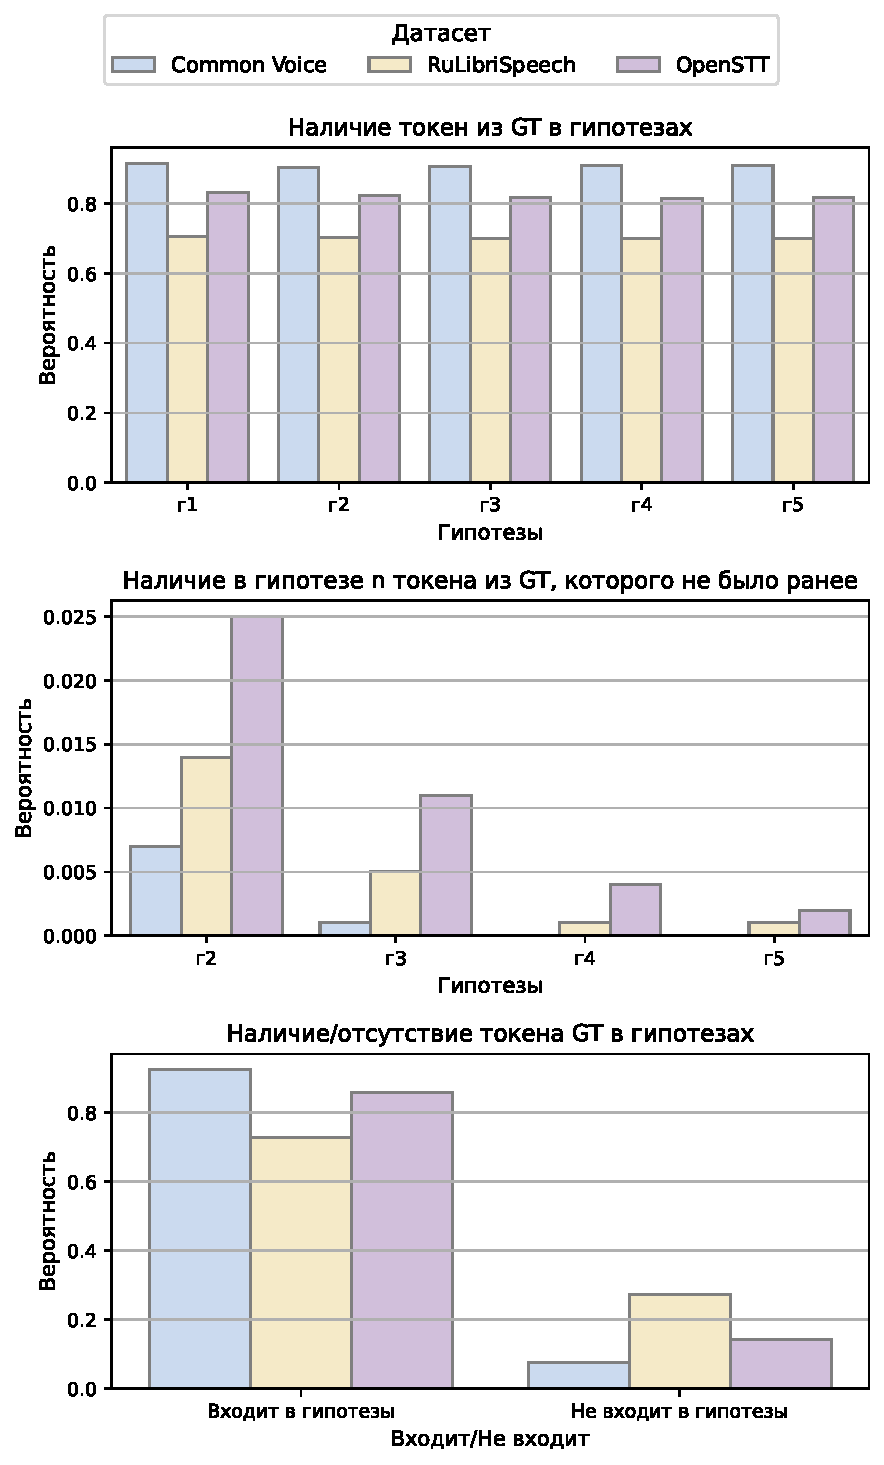
\includegraphics[width=100mm]{dist.pdf}
  \caption{Распределение токенов в сгенерированных датасетах}
  \label{fig:dist}
\end{figure}

Это та самая информация, которую наша модель может извлечь из сгенерированных гипотез и улучшить качество транскрипции.
Именно поэтом мы переходим к обучению отдельной языковой модели на ошибках.
Примеры из сгенерированного датасета представлены на листинге~\ref{lst:hypotheses}.
Здесь мы группируем информацию в JSON объекте.
По ключу «n\_best» мы получаем сгенерированные гипотезы.
По ключу «gt» же мы получим правильную транскрипцию, которую будем использовать в качестве цели для генерации во время обучения.
Данный формат был выбран из-за удобства использования в нашей задаче за счёт группировки в виде словарей.

\begin{lstlisting}[
  label={lst:hypotheses},
  caption={Пример структуры записи гипотез из тестового набора данных},
  breaklines=true,
  basicstyle=\small,
  keepspaces=true,
  escapechar=\%,
  frame=single,
]
{n_best: [
  %«Почему бы не положить конец конфиденциальности банковских операций?»%,
  %«почему бы не положить конец конфиденциальности банковских операций?»%,
  %«Почему бы не положить конец конфиденциальностей банковских операций?»%,
  %«Почему бы не положить конец конфиденциальностей банковских операций?»%,
  %«Почему бы не положить конец конфиденциальности банковских операций?»%
],
gt: %«Почему бы не положить конец конфиденциальности банковских операций?»%
} 
\end{lstlisting}

\section{Описание моделей и процесса обучения}

T5 (Text-to-Text Transfer Transformer)\cite{raffel2020exploring} -- это универсальная трансформерная модель, разработанная Google Research, которая переформулирует все задачи обработки естественного языка в единый формат Sequence-to-Sequence (Seq2Seq).
Её ключевая особенность -- подход, при котором задачи классификация, перевода, суммаризации и др. представляются как преобразование входной текстовой строки в выходную.

Модель использует энкодер-декодер структуру, где:
\begin{itemize}
  \item Энкодер обрабатывает входной текст, создавая контекстуализированные представления для каждого токена.
  В отличие от чисто декодерных моделей типа GPT, T5 использует двунаправленное внимание, что позволяет анализировать весь входной текст одновременно.
  \item Декодер генерирует выход последовательно, используя авторегрессионный механизм.
  При этом он учитывает скрытые состояния энкодера через кросс-внимание.
  Схожим образом работает ранее Whisper.
\end{itemize}

\begin{figure}[!t]
  \centering
  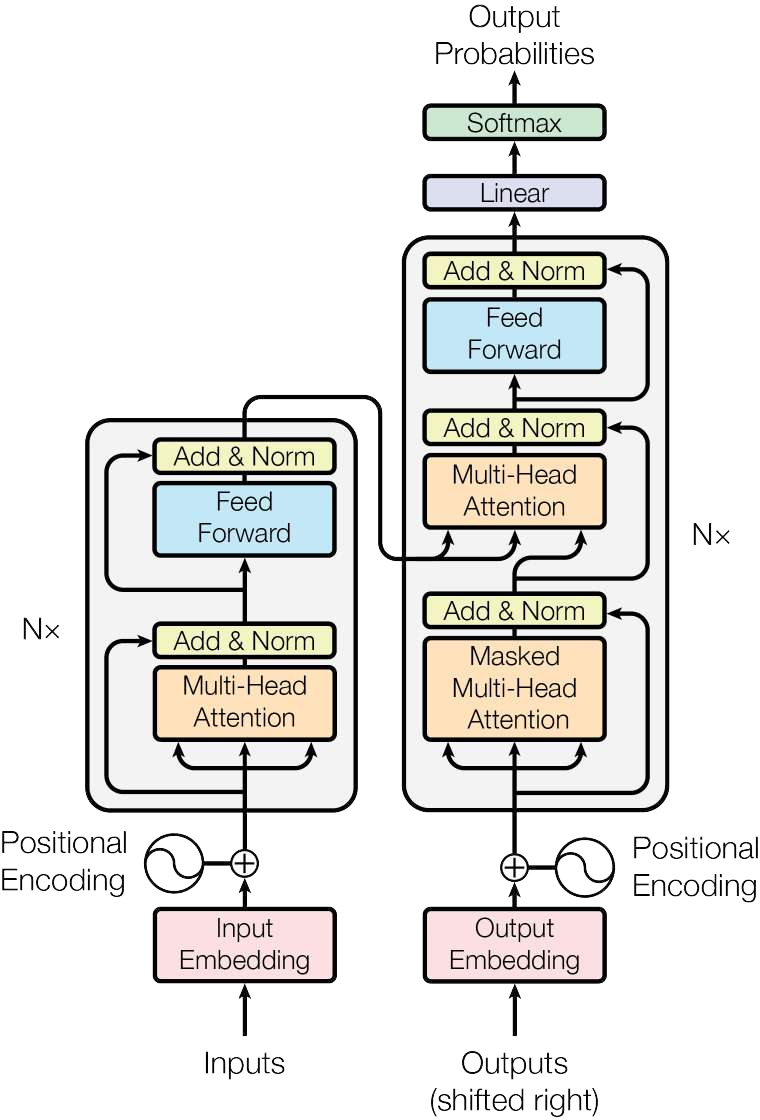
\includegraphics[width=80mm]{enc_dec.pdf}
  \caption{Архитектура энкодер-декодер}
  \label{fig:enc_dec}
\end{figure}

Схема архитектуры представлена на рисунке~\ref{fig:enc_dec}

Универсальность подхода Seq2Seq позволяет применять одну и ту же модель для десятков задач NLP без изменения архитектуры.
Мы сделаем ставку, что эта особенность позволит нам решить очевидную проблему со сдвигом между языками речевыми и рукописными.
Дело в том, что в повседневной речи люди могут использовать грамматически неправильные конструкции.
А с добавлением проблем с пропуском или вставкой слов от ASR, о которых мы говорили ранее, это может приводить к тому, что языковая модель может пытаться исправлять предложение на "более правильное" с точки зрения языка, но не с точки зрения того, что там было на самом деле.

В качестве двух моделей мы возьмём ruT5 и FRED-T5\cite{zmitrovich2023family}.
Обе модели были обучены Сбером на корпусе русского языка.
Они построены на архитектуре энкодер-декодер трансформеров.
Их мы выбрали по нескольким причинам:

\begin{enumerate}
  \item \textbf{Размер}.
  Мы берём Base (220М) и distill (95М) версии соответственно. 
  В паре с FastConformer это займёт немногим больше 3 Гб видеопамяти, что позволит влезть в любую пользовательскую видеокарту.
  \item \textbf{Архитектура}.
  Энкодер-декодер лучше улавливает ошибки и корректирует их.
  Такие выводы были сделаны на основе решения этой задачи для английского языка\cite{iudinenhancing}, где в качестве моделей-корректоров использовались Mistral-7b и Llama3-8b\cite{grattafiori2024llama}.
  На русском они также показывают плохие результаты, поэтому включены они не были.
\end{enumerate}

Обучение ruT5 будет проходить в few-shot сценарии, когда мы ей будем показывать 3 примера из валидационной выборке в качестве примера для улучшения.
Few-shot -- это подход, при котором языковая модель решает новую задачу, используя несколько демонстрационных примеров.
Математически это можно выразить как~\ref{eq:shot}:

\begin{equation}
  P(y_{test}|x_{test},\{x_i,y_i\}^K_{i=1}) = \prod_{t=1}^{T}P(w_t|w_{<t},x_{test},\{(x_i,y_i)\}^K_{i=1},\theta)
  \label{eq:shot}
\end{equation}
где $w_t$ - t-й токен ответа, $T$ - длина ответа, а $\theta$ - параметры модели.

Так мы проведём 15 обучающих эпох и сохраним модель с наименьшим WER на валидационной выборке.
Дополнительн мы используем алгоритм Low-rank adaptaion (LoRA)\cite{hu2022lora}.
Это подход к дообучению, при котором изначальные веса модели в выбранных слоях замораживаются и никак не изменяются в ходе дообучения.
В нашем случае такими слоями будут слои attention.
У каждой матрицы attention (Q, K, V, O) инициализируется своя пара матриц A и B размерами (d, rank) и (rank, h), где d и h – размер скрытого пространства матрицы attention, а rank – размер ранга, заданный при LoRA.
Во время обучения будут изменяться как раз матрицы A и B, которые как бы представляют собой сжатую информацию из весов слоя.
Преимуществом LoRA является то, что мы значительно экономим в используемой памяти, жертвуя качеством.
Это происходит благодаря тому, что в state оптимизатора хранятся не матрицы размера d $\times$ h, а две матрицы размеров d $\times$ rank и rank $\times$ h.
Баланс между памятью и качеством достигается за счёт настройки параметра ранга для LoRA.
Чем больше это значение, тем более точное представление изначального слоя мы получаем, но вместе с тем больше памяти будет храниться в state оптимизатора.
С формулой можно ознакомиться в уравнение~\ref{eq:lora}, а схему можно посмотреть на рисунке~\ref{fig:lora}:
\begin{equation}
  W_{new} = W_{frozen} + A \times B
  \label{eq:lora}
\end{equation}

\begin{figure}[!t]
  \centering
  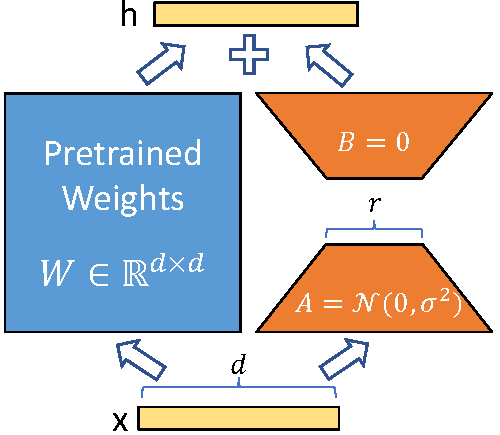
\includegraphics[width=70mm]{lora.pdf}
  \caption{Схема устройства подхода Low-rank adaptaion (LoRA)}
  \label{fig:lora}
\end{figure}

Использовался линейный планировщик с периодом разогрева.
Также стоит сказать, что модель обучалась исключительно на ошибках FastConformer модели.
Соответственно результаты для модели Whisper в связке с ruT5 будут показывать результат переноса способностей к коррекции между разными моделями в рамках одного набора данных.
Дополнительно было зафиксировано состояние псевдослучайного генератора, который использовался для перемешивания обучающих данных.
Это позволило лучше отслеживать, как изменения в настройках обучения влияло на качество коррекции, и повысило вопспроизводимость экспериментов.

Помимо обученного T5 мы применяли FRED-T5 дистилированный, который используется как инструмент для восстановления знаком препинания.
Это сделано для проверки способностей ASR моделей генерировать последовательности правильные с точки зрения пунктуации.

\begin{figure}[!t]
  \centering
  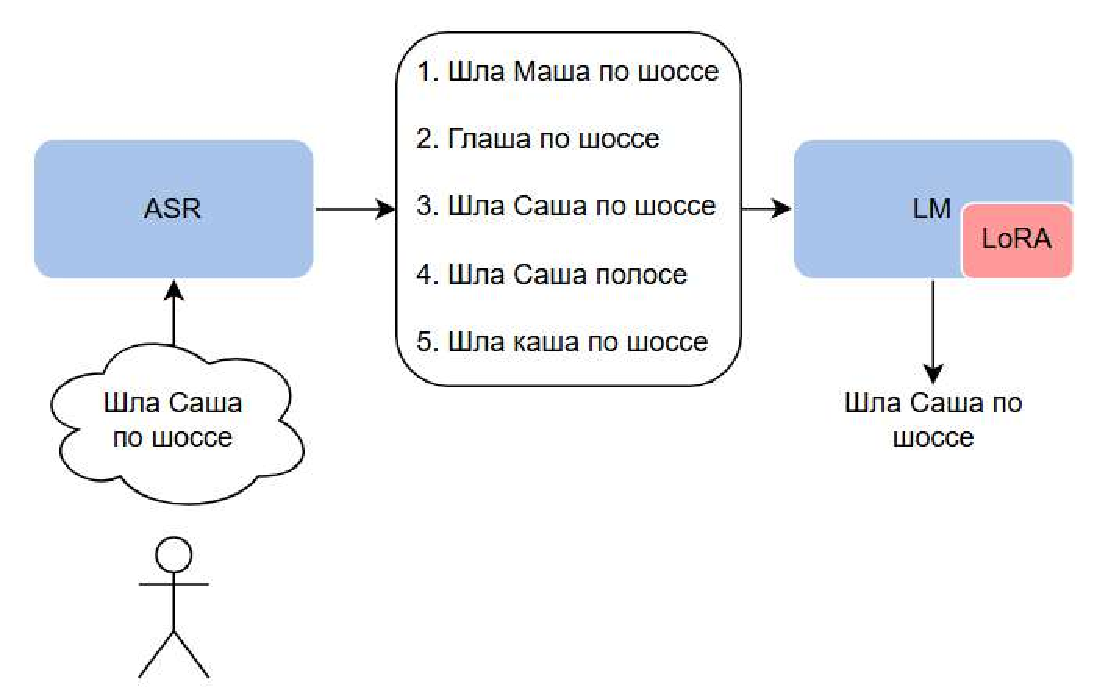
\includegraphics[width=120mm]{approach.pdf}
  \caption{Итоговая схема пайплайна}
  \label{fig:approach}
\end{figure}

Итоговую схему пайплайна можно изобразить как на рисунке~\ref{fig:approach}.
Кодом это можно выразить как едичный модуль.
В нём мы инициализируем две модели -- ASR и LM.
Если в качестве ASR мы берём FastConformer, то дополнительно необходимо поменять конфигурацию модели для генерации гипотез.
Затем обученный LoRA адаптер подгружаем к языковой модели и объединяем их.
Во время вызова пайплайна мы с помощью ASR и BeamSearch стратегии декодирования генерируем гипотезы.
На всякий случай дополнительно обрабатываем эти гипотезы, убирая пробелмы в начале и конце и два раза подряд идущие кавычки.
Группируем гипотезы вместе в словарь.
Передаём их в функцию по созданию промпта, которая добавит наши примеры из few-shot и токенизирует текст.
Получившийся вектор мы передаём в языковую модель, где с помощью BeamSearch мы генерируем исправленную транскрипцию.
Небольшая оговорка, что у ASR и LM конфигурации декодирования отличаются.
Для уменьшения шансов языковой модели выдать галлюцинацию, мы прописываем в её конфиге запрет на повторы токенов и предждевременную остановку декодирования.
Полученную последовательность токенов мы переводим в текст с помощью токенизатора и возвращаем из пайплайна.

\section{Результаты}

Результаты этой секции представлены двумя ветками экспериментов.
Первая исследует в целом способности модели к пост-коррекции на трёх наборах данных.
Вторая проверяет способности модели, обученной только на разнообразном Common Voice справляться с задачей.

\subsection{Основные результаты}
\begin{table}[]
\centering
\caption{Сравнение значений WER. ruT5 модель была дообучена на CV21 и RuLS}
\begin{tabular}{|c|c|ccc|}
\hline
\multirow{2}{*}{Модель}        & \multirow{2}{*}{Сеттинг}             & \multicolumn{3}{c|}{Датасет, WER}                                    \\ \cline{3-5} 
                               &                                      & \multicolumn{1}{c|}{CV21}  & \multicolumn{1}{c|}{RuLS}     & OpenSTT \\ \hline
\multirow{6}{*}{FastConformer} & Greedy                               & \multicolumn{1}{c|}{12.31} & \multicolumn{1}{c|}{38.43}    & 25.13   \\ \cline{2-5} 
                               & BeamSearch                           & \multicolumn{1}{c|}{12.26} & \multicolumn{1}{c|}{38.84}    & 25.07   \\ \cline{2-5} 
                               & LM                                   & \multicolumn{1}{c|}{9.87}  & \multicolumn{1}{c|}{37.18}    & 27.28   \\ \cline{2-5} 
                               & Greedy+Distill                       & \multicolumn{1}{c|}{13.81} & \multicolumn{1}{c|}{42.16}    & -       \\ \cline{2-5} 
                               & BeamSearch+Distill                   & \multicolumn{1}{c|}{11.82} & \multicolumn{1}{c|}{42.10}    & -       \\ \cline{2-5} 
                               & BeamSearch+ruT5                      & \multicolumn{1}{c|}{9.75}  & \multicolumn{1}{c|}{34.32}    & 23.81   \\ \hline
\multirow{4}{*}{Whisper}       & Greedy                               & \multicolumn{1}{c|}{19.60} & \multicolumn{1}{c|}{37.89}    & 24.38   \\ \cline{2-5} 
                               & BeamSearch                           & \multicolumn{1}{c|}{18.33} & \multicolumn{1}{c|}{35.49}    & 24.19   \\ \cline{2-5} 
                               & Greedy+Distill                       & \multicolumn{1}{c|}{20.57} & \multicolumn{1}{c|}{41.40}    & -       \\ \cline{2-5} 
                               & BeamSearch+ruT5                      & \multicolumn{1}{c|}{14.32} & \multicolumn{1}{c|}{32.48}    & 23.90   \\ \hline
\end{tabular}
\label{tab:res_full}
\end{table}

Проанализируем результаты таблицы~\ref{tab:res_full}.
Как мы видим, во всех случаях наш алгоритм превзошёл альтернативные подходы и уменьшил ошибку.
В среднем, мы уменьшаем WER на 2-3 \% для FastConformer и либо приводим транскрипции по качеству к Whisper, несмотря на то, что FastConformer+ruT5 занимают около 400 миллионов параметров, либо значительно его обходим.
Также здесь мы отлично наблюдаем эффект переноса обучения коррекции между разными ASR, потому что наш подход успешно исправляет ошибки у Whisper.
И это при том, что ruT5 обучалась исключительно на транскрипциях FastConformer.
Это значит, что подход по объединению богатых лингвистических знаний языковой модели и дообучения под нашу задачу работает отлично.

Наибольшей репрезентативность обладает датасет Common Voice.
Можно так утверждать, поскольку этот набор данных содержит наибольшим количеством тем и спикеров с акцентами.
Вместе с тем к нему меньше всего вопросов в плане пунктуации, особенно после предобработки, о которой мы говорили ранее.
На нём мы видим, что модель Whisper гораздо лучше справилась с передачей пунктуации, чем FastConformer.
Это понятно, благодаря эксперименту с FRED-T5 Distill, который как раз специализируется на исправлениях слов и пунктуации в предложениях.
Поскольку его результаты на Common Voice 21 у модели Whisper показывают больше ошибку, она скорее испортила предложения.
У FastConformer в этом плане ситуация сложнее, при жадном декодирование FRED также увеличил значение среднего WER, однако при декодирование со стратегией BeamSearch удалось выиграть 0.4 пункта.
Если же концентрироваться на результатах, то ruT5 принесла повышение точности на 2.5 пункта для FastConformer и 4 для Whisper.
Это хороший прирост при учёте малой дополнительной вычислительной нагрузки, которую несёт алгоритм.
И ещё это интересная деталь -- модель спрвилась с Whisper лучше, хотя обучалась на FastConformer.
Но это может быть следствием того, что в целом WER у ASR от OpenAI выше изначально.

С RuLibriSpeech, который назван RuLS в таблице, ситуация немного сложнее.
Как уже обсуждалось в начале прошлой главы, этот датасет содержит записи аудиокниг.
Несмотря на то, что у текстовой аннотации есть реальный исходник, у которого проблем с пунктуацией быть не должно, в RuLibriSpeech всё равно встречаются такие предложения.
Для примера возьмём одно из первых предложений из тестового набора:
«Ничьих не требуя похвал, Счастлив уж я надеждой сладкой, Что дева с трепетом любви Посмотрит, может быть украдкой, На песни грешные мои. У лукоморья дуб зеленый».
Здесь сразу две проблемы.
Во-первых -- предложение изначально было разбито на по строкам, из-за чего у нас такое смешивание верхнего и нижнего реистра.
Во-вторых -- в конце предложения нет точки.
Как итог, этот датасет обладает самым большим значением WER среди всех трёх.
Дополнительно мы видим, что модель FRED на этом наборе данных во всех случаях только ухудшает итоговый результат.
Причина может заключаться в том, что модель как раз исправляет пунктуацию в сгенерированных аудио, из-за чего идёт большое расхождение с первоисточником.
Также стоит заметить что, казалось бы, BeamSearch алгоритм, который при генерации выбирает самую вероятную последовательность, проигрывает жадному декодированию в FastConformer.
Случился как раз редкий момент, когда greedy оказался более успешным.
Несмотря на эти проблемы, наша модель, в том числе обученная  и на тренировочной часте этого набора данных, справилась с поставленной задачей.
Уменьшение WER на 5 и 3 пунктов для FastConformer и Whisper говорит, что даже такие проблемы, как пунктуация, в целом могут быть невелированы пост-коррекцией.

OpenSTT набор ютуба также имеет несколько нюансов.
\begin{enumerate}
  \item Его транскрипции были переведены в нижний регистр.
  \item Из его предложений была убрана вся пунктуация.
\end{enumerate}

В силу этих двух причин мы не обучали нашу модель на обучающем сплите датасета.
И по той же причине мы не рассматриваем варианты с FRED, поскольку в добавление пунктуации в случае, когда она будет убрана, смысла нет.
Для соотвествия такому варианту форматирования, мы с помощью регулярных выражений вырезали из генерации только слова и цифры и привели текстовые знаки к нижнему регистру.
Здесь мы видим самую маленькую величину прироста.
Для модели от OpenAI она составляет всего 0.2 пукта, а для ASR от Nvidia 1.2.
Но во-первых -- прирост всё-таки есть.
А во-вторых -- большая часть неправильных генераций может быть вызвана как раз тем, что ruT5 была больше заточена под предложения с пунктуацией.
Соответственно и генерировала исправления она с учётом пунткуации в частности и семантики языка в целом.
Отсюда мы и видим настолько невоодушевляющие результаты.

Примеры генераций можно найти в таблице~\ref{tab:ex}.
Как мы можем здесь видеть, WER метрика может выдавать значения, которые не легко осознаются.
Так расстояние Левенштейна между «время» и «время.» составляет единицу, поскольку мы получаем одно правильное слово $C$ и одну вставку $I$ из-за точки.

\begin{table}[]
  \centering
  \caption{Примеры работы алгоритма пост-коррекции на наборе аудио \\данных Common Voice 21}
  \label{tab:ex}
\begin{tabular}{|c|c|c|c|}
\hline
ASR                                                                                            & \begin{tabular}[c]{@{}c@{}}ASR\\ WER\end{tabular} & LM                                                                                             & \begin{tabular}[c]{@{}c@{}}LM\\ WER\end{tabular} \\ \hline
Я знаю, я все знаю.                                                                            & 20                                                & Я знаю, я всё знаю.                                                                            & 0                                                \\ \hline
\begin{tabular}[c]{@{}c@{}}Я сейчас догоню тебя.\\ Крикнул он Яшвину.\end{tabular}             & 37.5                                              & \begin{tabular}[c]{@{}c@{}}Я сейчас догоню тебя, –\\ крикнул он Яшвину.\end{tabular}           & 12.5                                             \\ \hline
\begin{tabular}[c]{@{}c@{}}Зачем я стараюсь,\\ дружусь?\end{tabular}                           & 25                                                & \begin{tabular}[c]{@{}c@{}}Зачем я стараюсь,\\ тружусь?\end{tabular}                           & 0                                                \\ \hline
\begin{tabular}[c]{@{}c@{}}Четвертый герой\\ десятка сражений.\end{tabular}                    & 40                                                & \begin{tabular}[c]{@{}c@{}}Четвертый -- герой\\ десятка сражений.\end{tabular}                 & 20                                               \\ \hline
\begin{tabular}[c]{@{}c@{}}Вам, завещаю я,\\ сад фруктовый моей\\ великой души.\end{tabular}   & 37.5                                              & \begin{tabular}[c]{@{}c@{}}Вам завещаю я\\ сад фруктовый моей\\ великой души.\end{tabular}     & 0                                                \\ \hline
\begin{tabular}[c]{@{}c@{}}Вам здесь лучше,\\ чем по-прежнему\\ флигельке.\end{tabular}        & 42.86                                             & \begin{tabular}[c]{@{}c@{}}Вам здесь лучше,\\ чем в прежнем\\ флигельке.\end{tabular}          & 14.28                                            \\ \hline
время                                                                                          & 0                                                 & время.                                                                                         & 100                                              \\ \hline
\begin{tabular}[c]{@{}c@{}}Еще печальнее\\ отношения гения\\ к специалистам.\end{tabular}      & 0                                                 & \begin{tabular}[c]{@{}c@{}}Еще печальнее\\ отношение гения\\ к специалистам.\end{tabular}      & 16.66                                            \\ \hline
\begin{tabular}[c]{@{}c@{}}Глаза глядели\\ все так же странно.\end{tabular}                    & 0                                                 & \begin{tabular}[c]{@{}c@{}}Глаза глядели\\ всё так же странно.\end{tabular}                    & 16.66                                            \\ \hline
Эй, это я. Кто ты?                                                                             & 60                                                & Эй, это я, кто ты?                                                                             & 80                                               \\ \hline
\begin{tabular}[c]{@{}c@{}}Наверное, пошел\\ сделать предложение\\ отцу Леонарду.\end{tabular} & 0                                                 & \begin{tabular}[c]{@{}c@{}}Наверное, пошел\\ сделать предложение\\ отцу Леонардо.\end{tabular} & 16.66                                            \\ \hline
\end{tabular}
\end{table}


\subsection{Обучение исключительно на CommonVoice}
\begin{table}[]
\centering
\caption{Сравнение значений WER. ruT5 модель была обучена исключительно на CV21}
\begin{tabular}{|c|c|ccc|}
\hline
\multirow{2}{*}{Модель}        & \multirow{2}{*}{Сеттинг}             & \multicolumn{3}{c|}{Датасет, WER}                                    \\ \cline{3-5} 
                               &                                      & \multicolumn{1}{c|}{CV21}  & \multicolumn{1}{c|}{RuLS}     & OpenSTT \\ \hline
\multirow{2}{*}{FastConformer} & BeamSearch                           & \multicolumn{1}{c|}{12.26} & \multicolumn{1}{c|}{38.34}    & 25.07   \\ \cline{2-5} 
                               & BeamSearch+ruT5                      & \multicolumn{1}{c|}{3.20}  & \multicolumn{1}{c|}{40.07}    & 23.38   \\ \hline
\multirow{2}{*}{Whisper}       & BeamSearch                           & \multicolumn{1}{c|}{18.33} & \multicolumn{1}{c|}{35.49}    & 24.19   \\ \cline{2-5} 
                               & BeamSearch+ruT5                      & \multicolumn{1}{c|}{4.99}  & \multicolumn{1}{c|}{38.04}    & 23.91   \\ \hline
\end{tabular}
\label{tab:res_cv_trained}
\end{table}

Ещё одной веткой экспериментов было обучение исключительно на русской части Common Voice 21.
Здесь мы проверяли, насколько хватит самого разнообразного набора для нашей задачи в целом.

Взглянув на таблицу~\ref{tab:res_cv_trained}, мы можем сделать несколько выводов.
Начнём с того, что на 2/3 датасетах мы всё равно получили прирост.
Более того, на Common Voice мы достигли уменьшения значения ошибки в 3-4 раза на обеих системах ASR.
Это значительный прирост, но мы стоит посмотреть, что на других наборах результаты не такие замечательные.
Поскольку, как говорилось ранее, Common Voice по нескольким причинам можно считать самым репрезентативным, это можно назвать успехом.

С OpenSTT ситуация немного похуже.
Величина уменьшения ошибки тут >1, что стало ещё хуже, чем было при обучение на Common Voice + RuLibriSpeech.
Это может указывать на большой domain shift между этими наборами данных, который частично компенсировался за счёт аудиокниг.
Природу этого искажения сложно осмыслить.
Но можно предположить, что это случилось из-за того, что OpenSTT и RuLibriSpeech разделяют общие проблемы с пунктуацией.

RuLibriSpeech же показал ухудшение показателей.
Это по большей части связано как раз ранее описанными проблемами с пунктацией.
Без примеси этого рода ошибок в обучающем наборе данных, модель старается делать коррекцию на манер Common Voice, где эти проблемы сильно менее выражены.

\section{Ограничения}

Логично, что у нашей системы есть единая точка отказа.
Мы зависим от качества распознавания ASR.
Если галлюцинации языковой модели можно невелировать тем, что мы можем дополнительно сохранять расшифровки ASR, то вот в случае ошибок на стороне модели распознавания речи, мы сильно теряем в итоговом качестве.

Для оценки влияния этой проблемы и общей устойчивости системы, были проведены эксперименты с зашумлением аудио.
Строго говоря, данные эксперименты можно проводить с разными видами аугментаций аудио, которых существует очень много.
Как минимум можно назвать гауссовский шум, высоко- и низкочастотные фильтры, изменение высоты тона, фоновые шумы, импульсный отклик помещения (RIR) и другие.
Для последних двух даже существуют отдельные наборы со звуками, которые хорошо интегрируются с экосистемой PyTorch.
Однако мы пойдём по пути более целенаправленного изменения аудио -- с использованием состязательных атак (adversarial attacks)\cite{olivier2022recent,zhang2022adversarial,carlini2018audio}.

Состязательными атаками называют небольшие, но тщательно подобранные изменение в подаваемых в модель данных таким образом, чтобы сама модель думала, будто бы данные имеют другое значение.
В то время, как аугментация улучшает обобщающие сопобности, использование состязательных атак улучшают устойчивость к оптимизированным малозаметным изменениям.
Сами эти изменения могут даже быть незаметными для человека, однако нейронные сети при виде их начинают значительно ошибаться.
Из банальных примеров -- изменение картинки с цифрой 1 таким образом, чтобы модель думала, что там цифра 7\cite{warr2019strengthening}.
Или же, в нашем случае, что в аудио было сказано нечто другое.
Сами атаки бывают двух видов:

\begin{itemize}
  \item White-box attack, когда мы знаем архитектуру модели и имеем непосредственный доступ её выходу.
  Это возможно, если модель развёрнута на инфрастуктуре, к которой мы имеем доступ.
  Поскольку мы используем модели локально, мы далее будем использовать атаки из этой группы.
  \item Black-box attack, когда мы не знаем архитектуру модели.
  Допустим, мы обращаемся к ней по API и получаем сразу текст.
  Из примеров можно вспомнить ChatGPT, от которого мы на наши запросы сразу получаем ответ.
\end{itemize}

Типов атак существует очень много.
Их можно также разбить на целевой и нецелевой.
В первой группе атаки, при использование которых мы пытаемся изменить данные таким образом, чтобы модель предсказывала определённое значение.
Алгоритмами из второй группы мы изменяем изначальные данные таким образом, чтобы модель ошибалась, а как именно нам не важно.
Далее мы будем оперировать градиентными атаками, а значит относящимися к группе целевых, потому что, чтобы посчитать градиент, нам нужно целевое предсказание и функция потерь.

Самым базовым алгоритмом состязательных атак является Fast Gradient Sign Method (FGSM).
FGSM -- одна из самых известных состязательных атак, предложенная Яном Гудфелоу в 2014 году\cite{goodfellow2014explaining}.
Это простая, но эффективная white-box атака, использующая градиенты модели для создания adversarial-примеров.
Как мы знаем - градиент указывает направление возрастания функции.
Во время обучения, мы берём антиградиент, чтобы идти в направление убывания функции потерь и меняем веса модели.
Однако, сам градиент можно использовать, чтобы определить направление, в котором изменения в данных приведут к максимальному увеличению ошибки модели.
Сами же веса модели остаются нетронутыми.
Формула атаки FGSM представлена в уравнение~\ref{eq:fgsm}:

\begin{equation}
  x_{adv} = x + \alpha sign \nabla_x L(f(x), y_{target})
  \label{eq:fgsm}
\end{equation}
где $\alpha$ - величина изменений, $\nabla$ - градиент функции потерь, $f(x)$ - модель ASR, которая принимает аудио и возвращает логиты.

Благодря FGSM мы можем за один шаг получить возмущения в аудио.
Но если подумать, то когда мы обучаем модель, мы же делаем кучу шагов в направление минимума.
Что нам мешает делать кучу шагов в направление максимума, но с ограничением размера максимального шага?
Как выяснилось, ничего.
Так был придуман Projection Gradient Descent (PGD)\cite{madry2017towards}.

PGD -- это итеративный алгоритм оптимизации, применяемый для задач с ограничениями на параметры.
Он сочетает идеи градиентного спуска с проекцией на допустимое множество.
PGD расширяет классический градиентный спуск, добавляя шаг проекции после каждого обновления параметров.
Если градиентный спуск просто двигается в направлении антиградиента, то PGD дополнительно «проецирует» новую точку обратно на допустимое множество, если та вышла за его пределы.
Это позволяет контролировать свойства модели, такие как устойчивость к атакам или физическую осмысленность параметров.
PGD решает задачу атаки итеративно, комбинируя градиентный подъём (для увеличения потерь) и проекцию (для соблюдения ограничений).
Таким образом генерируется шум на аудио.

Пошагово его можно расписать следующим образом:
\begin{enumerate}
  \item Задаются начальные гиперпараметры PGD.
  Их у нас 3: максимальная величина изменений амплитуды, размер шага и количество шагов.
  \item Задаётся соревновательная транскрипция, к которой мы будем итерироваться.
  В нашем случае я выбрал простую фразу «вас взломали».
  \item В качестве одного шага мы пропускаем аудио через модель.
  \item Аудио затем изменяется на величину изменения и знак градиента.
  \item Амплитуда затем обрезается сначала по значению максимальной величины изменения, а затем и в диапозоне [-1, 1].
  Данные значения обрезания используется изменной для аудио.
  Для изображения мы бы скорее использовали [0, 1].
  \item После всех итераций мы получаем зашумлённое аудио.
\end{enumerate}

Формулу PGD можно выразить как~\ref{eq:pdg}:

\begin{equation}
  x_{t+1} = clip_{|1|, \epsilon}(x_t + \alpha sign \nabla_x L_{CTC}(f(x_t), y_{target}))
  \label{eq:pdg}
\end{equation}
где $t$ - номер шага, $\epsilon$ максимальная величина изменений амплитуды, $\alpha$ - величина шага, $\nabla$ - градиент функции потерь, $L_{CTC}$ - фукнция потерь CTC, $f(x)$ - модель ASR, которая принимает аудио и возвращает логиты.

Возвращаясь к вопросу «Почему состязательные атаки, а не аугментации?» отвечу на него так «Мы хотим явно проверить сопротивляемость системы злонамеренным искажениям».
Состязательные атаки создают наиболее опасные возмущения, которые сложнее всего распознать.
Артефакты, которые они порождают атаки, могут лучше отражать естественные искажения в аудио, которые пораждают плохой микрофон, окружающие шумы и прочее\cite{engstrom2019adversarial}.

Мы намерено атаковали ASR Whisper с помощью PGD и функцией потерь CTC в авторегрессионном режиме.
Набором данных выступят 2000 аудио из Common Voice, который мы отберём случайным образом.
Генераторы псевдослучайных чисел Python, NumPy и PyTorch были зафиксированы перед проведением эксперимента для воспроизводимости.
Таким образом аудио, которые отбирались для состязательных атак, были бы одни и те же в случае, если бы мы захотели поменять параметры атаки.

\begin{table}[]
\centering
\caption{Эксперимент с Projected Gradient Descent white-box атакой на модель Whisper на датасете Common Voice}
\begin{tabular}{|c|c|c|}
\hline
Модель                         & Сеттинг                              & WER     \\ \hline
\multirow{2}{*}{Whisper}       & BeamSearch                           & 24.48   \\ \cline{2-3} 
                               & BeamSearch+ruT5                      & 21.34   \\ \hline
\end{tabular}
\label{tab:pgd}
\end{table}

Первое, что мы видим -- мы повысили значение ошибки на треть за счёт атаки.
Как итог, WER достигает 24 пунктов.
Второе -- наш алгоритм всё равно способен улучшить в таком случае транскрипцию аудио.
Да, если сравнивать этот эксперимент с похожим по обучению исключительно на Common Voice, у нас наблюдается не настолько впечатляющее уменьшение ошибки.
Если там WER уменьшался в несколько раз, то тут всего на 1/8.
Однако стоит понимать, что здесь изначальные аудио в целом обладают более низким качеством.
Дополнительно ruT5 на зашумлённых аудио мы не тренировали, то есть здесь языковая модель, обученная на чистых записях, которые были прогонены через FastConformer.
Значит мы наблюдаем прирост одновременно и при переносе знаний о коррекции между ASR, и при ухудшение качества аудио.
Не стоит ждать магического превращения абсолютно неверных транскрипций в правильные, однако некоторые ошибки мы всё равно способны исправлять.

По итогу можно сказать, что подход по корекции транскрипций справляется с поставленной задачей.

Конечно, всё ещё остаётся риск того, что языковая модель может сама ухудшить транскрипцию.
Вот пример из Commmon Voice 21: «Полине было предложено использовать эти примеры в качестве аргументов для следующих гипотез.».
Эта проблема невелируется тем, что мы можем дополнительно сохранять расшифровки речи из модели ASR.

Также ограничением является распознавание речи в реальном времени.
Сложность здесь завязана на том, что мы дважды применяем генерацию с BeamSearch стратегией -- внутри ASR и внутри LM.
В такой конфигурации использование системы пост-коррекции для задачи распознавания речи в реальном времени может не соответствовать необходимым требованиям.
Ещё проблемой сверху выступает выравнивание речи.
В real-time системах аудио обычно разбивается на отрезки и по ним уже распознаётся.
Для повышения точности, в новый кусочек также закладывается часть от прошлого.
Если в случае ASR задача уже не простая, то при добавление языковой модели мы не просто согласуем отдельные кусочки распознавания, но должны учитывать 5 потенциальных расшифровок.
Вопросы «Стоит ли нам менять транскрипцию, если LM выбрала токен из другой гипотезы?» и «Что, если она вновь поменяла мнение?» являются на данный момент ключевыми в данном вопросе и требуют дальнейшего исследования.

\section{Дополнительные эксперименты}

Были проведены дополнительные эксперименты с NEFTune\cite{jain2023neftune} и текстовой аугментацией.
Поговорим сначала про NEFTune.

\subsection{NEFTune}
Он представляет собой метод регуляризации, разработанный для улучшения процесса дообучения языковых моделей.
Его ключевая особенность заключается во внесении контролируемого гауссовского шума к эмбеддингам входных токенов перед их подачей в модель на этапе обучения, что способствует повышению устойчивости и обобщающей способности модели.
Этот подход особенно эффективен при работе с ограниченными наборами данных для дообучения.

Математически это выражается как модификация исходного векторного представления через добавление случайного вектора, элементы которого распределены по нормальному закону.

\begin{equation}
  \begin{aligned}
    &\epsilon \sim Uniform(-1, 1) \\
    &X'_{emb} = X_{emb} + (\frac{\alpha}{\sqrt{Ld}})\cdot\epsilon  
  \end{aligned}
  \label{eq:neftune}
\end{equation}
где $L$ и $d$ - размерности вектора, а $\alpha$ - задаваемая величина шума.

Для успешного использования NEFTune необходимо тщательно подбирать уровень шума.
Слишком интенсивное зашумление может ухудшить качество модели, тогда как недостаточное - не даст желаемого регуляризирующего эффекта.
Оптимальные значения параметра шума обычно находятся в относительно узком диапазоне, авторы проверяли диапозон [5, 15].
Экспериментально установлено, что этот подход демонстрирует наибольшую эффективность при работе с небольшими наборами данных для дообучения.
Однако настройка уровня шума вместе с тем и является главным недостатком NEFTune.
Метод требует тщательного подбора параметра шума, что может увеличивать время настройки модели.
Также отмечается незначительное увеличение времени обучения из-за дополнительных операций генерации и добавления шума.

В стандартном процессе обучения по большей части ничего не меняется.
Модель продолжает использовать стандартную функцию потерь и немодифицированный алгоритм обратного распространения ошибки.
Однако перед каждым прямым проходом к входным эмбеддингам добавляется шумовой компонент, то есть эмбеддинга вычисляется его зашумленная версия.
Важно отметить, что эта операция выполняется исключительно на этапе обучения, тогда как при инференсе модель работает с исходными, незашумленными представлениями.
Такой подход обеспечивает сохранение производительности модели в рабочих условиях.

Добавление шума выполняет несколько полезных функций в процессе обучения.
Во-первых, оно действует как дополнительный регуляризатор, предотвращая переобучение модели на специфичных особенностях небольшого обучающего набора.
Во-вторых, шум способствует сглаживанию ландшафта оптимизируемой функции, помогая алгоритму избегать локальных минимумов.
В-третьих, каждый пример в эпоху обучения получает уникальную шумовую добавку, что косвенно увеличивает разнообразие обучающих данных.

По сравнению с традиционными методами регуляризации, NEFTune обладает рядом преимуществ.
В отличие от dropout, который воздействует на активации скрытых слоев, он работает непосредственно с входными представлениями.
Благодаря этому не происходит поломок графа  и перекомпиляций.
В сравнении с weight decay, который глобально ограничивает величину параметров, NEFTune обеспечивает более тонкое и адаптивное регулирование процесса обучения.
При этом метод сохраняет простоту реализации и не требует значительных вычислительных ресурсов.
Кроме того, данный подход принёс прирост качества в аналогичной работе для английского языка

\subsection{Текстовая аугментация}
Нашие текстовые аугментации будут симулировать ошибки ASR, которые мы обсуждали ранее: удаление и вставка случайных слов.
Мы выберем 10\% набора данных Common Voice, применим к ним аугментации, остальные 90\% оставим как есть и обучим модель.

Симуляция пропуска слов в своей реализации достаточно простая, поэтому начнём с неё.
Мы разбиваем предложение по пробелам на отдельные слова, удаляем случайное и объединяем оставшиеся слова обратно.
Со вставкой ситуация более сложная.

Мы переведём задачу вставки случайного слова в парадигму задачи заполнения маски (fill-mask).
Fill-Mask -- это задача предобучения языковых моделей, где система учится предсказывать пропущенные или замаскированные слова в тексте.
Она лежат в основе современных трансформерных моделей, таких как BERT\cite{devlin2019bert}, и позволяют эффективно обучать модели понимать контекст и семантику языка.
Мы же будем пытаться наоборот отучить модель от семантической правильности языка и таким образом попробуем решить проблему с тем, что модель может менять предложения исходя не из звучания, но из правил правописания.

Принцип работы маскирования заключается в том, что мы заменяет токен текста на специальный токен маски [MASK], а модель должна восстановить оригинальные слова. В BERT обучение реализовано следующим образом:
\begin{itemize}
  \item Входной текст разбивается на токены.
  \item 15\% токенов заменяются на [MASK] (80\% вероятность), случайное слово (10\%) или остаются без изменений (10\%).
  \item BERT, на основе механизма двунаправленного внимания, благодаря которому на обучающей выборке выучиваются взаимосвязи между токенами, начинает предсказывать значение слова за токеном [MASK].
  \item Считается ошибка кросс-энтропией с учётом масок.
\end{itemize}

BERT идеально подходит для Fill-Mask.
За счёт двунаправленного внимания он анализирует весь контекст вокруг маски, а не только предыдущие слова, как было бы в GPT.
Это позволяет точнее предсказывать пропущенные слова.  
Недостатком можно выделить, что если в тексте несколько масок, BERT обрабатывает их независимо, не учитывая взаимное влияние.  

Собвственно по аналогии с удалением, мы разобьём предложение по словам, вставим в случайное место токен [MASK] и с помощью BERT заполним его.
Единственная оговорка - мы будем использовать RuBERT\cite{zmitrovich2023family}, также обученный Сбером, как и ruT5 и FRED-T5.
Его мы выбираем из-за того, что он был обучен на большом корпусе русского текста и лучше должен вставлять слова, подходящие по контексту.

За счёт этих двух текстовых аугментаций мы попытаемся заставить ruT5 меньше полагаться на семантическую логику языка, которая может отсутствовать в речи.

\subsection{Результаты дополнительных экспериментов}

\begin{table}[]
\centering
\caption{Эксперимент с аугментированием гипотез с целью улучшить качество генерации}
\begin{tabular}{|c|c|c|}
\hline
Модель                         & Сеттинг                              & WER     \\ \hline
\multirow{3}{*}{FastConformer} & BeamSearch                           & 12.26   \\ \cline{2-3} 
                               & BeamSearch+ruT5 (neft)               & 169.94  \\ \cline{2-3} 
                               & BeamSearch+ruT5 (aug)                & 71.42   \\ \hline
\multirow{3}{*}{Whisper}       & BeamSearch                           & 18.33   \\ \cline{2-3} 
                               & BeamSearch+ruT5 (neft)               & 168.90  \\ \cline{2-3} 
                               & BeamSearch+ruT5 (aug)                & 79.52   \\ \hline
\end{tabular}
\label{tab:fails}
\end{table}

Результаты дополнительных экспериментов представлены в таблице~\ref{tab:fails}.
Как мы видим, данные эксперименты не увенчались успехом.

NEFTune даже при выставление маленького значения $\alpha$ для генерируемого гауссовского шума всё равно очень сильно шумил модель.
Поскольку данный метод регуляризации разботал для больших моделей типа GPT\cite{jain2023neftune}, а также для модели с архитектурой T5 в похожей задачи\cite{iudinenhancing}, можем предположить, что проблема в размере модели.
Возможно, зашумление для модель столь маленького размера привело к тому, что мы не смогли между при передаче информации между слоями не смогли обучиться вычлинять информацию.
Использование модели большего размера в теории могло бы принести прирост, однако это скорее тема будущих исследований проблемы.

Текстовые аугментации также принесли лишь рост ошибки.
Это может быть вызвано тем, что при удаление слов в предложение в обучающей выборке, мы теряли в большинстве случаев правильные токены.
Таким образом мы заставляли модель галюционировать, то есть генерировать какие-то токены, которых в изначальной последовательности не было.

\section{Анализ производительности}
Как было написано в части про выбор модели, одной из задач выступало низкоресурсное использование.
При обучение контроль ресурсов сводится к балансированию нескольких факторов:

\begin{itemize}
  \item Используемый тип данных для весов модели и/или активаций.
  Мы можем квантовать модель\cite{lin2024awq} или использовать смешанную точность при прямом проходе\cite{micikevicius2017mixed}.
  Первый вариант значительно снижает потребление памяти, но вредит качеству.
  При нём мы переводим все веса модели в другой тип данных (int8, int4, normal float4) и теряем в точности.
  Второй незначительно вредит качеству и незначительно уменьшает затраты памяти.
  При нём мы считаем наши активации с пониженной точностью (float16 или bfloat16\cite{kalamkar2019study}) и затем перед обратным распространением возвращаемся к полной точности (float32).
  \item Ранг LoRA.
  Как говорилось в части про LoRA, мы можем изменить ранг и, таким образом, уменьшить размеры матриц A и B.
  Вместе с тем мы уменьшим точность репликации оригинальных модулей.
  Стоит при этом не забывать, что в таком случае рекомендуется уменьшить ещё и параметр $\alpha$.
  Обычно его делают равным или в два раза больше или меньше значения ранга.
  Также можно попробовать другие подходы через оптимизацию графа вычислений\cite{cherniuk2023run}.
  \item Реализация механизма внимания.
  T5 модель поддерживает использования Scaled Dot-Product Attention (SDPA)\cite{dao2022flashattention,dao2023flashattention} из коробки, что может уменьшить потребление памяти на современных видеокартах.
  \item Изменение размера batch'а вплоть до одного примера.
  В данном случае можно компенсировать его за счёт аккумуляции градиента, равной делению изначального размера на уменьшенный.
\end{itemize}

При инференсе, то есть непосредственном использование моделей, можно также применить алгоритмы понижения точности за счёт квантования.
И ещё можно протестировать SDPA.
Однако в этом нет особой необходимости, поскольку по итогу обе модели вместе занимают порядка 3 Гб видеопамяти при том, что 4 Гб является минимумом для пользовательских видеокарт последних лет пяти.

Касательно скорости, самым простым способом уменьшить количество вычислений - объединить обученный адаптер LoRA и модель ruT5.
Делается это одной простой функцией после загрузки обеих частей в коде.
Также не стоит забывать о переводе модели в режим оценки и использование no\_grad контекста, благодаря которым прямой проход будет получаться быстрее.
Дополнительно действенным алгоритмом действий, начиная с версии PyTorch 2.0, является компиляция графа вычислений.
FastConformer и ruT5 можно объединить в рамках одного модуля и скомпилировать, тем самым мы получим единый граф.
В таком случае общая система занимает 2.932 Гб видеопамяти и утилизирует H100 на 77\%.
Из них ASR от Nvidia занимает 1.224 Гб и утилизирует 39\%, а LM от Сбера - 1.708 Гб и 46\% соответственно.
На аудио длиной 7 секунд в среднем генерация транскрипций занимает примерно 2.3 секунды.
Из этого времени 1.2 занимает генерация гипотез с FastConformer и 0.6 коррекция этих самых гипотез.
Как итог мы видим, что дополнительная нагрузка из-за языковой модели по времени всего на треть больше времени работы ASR, по памяти и утилизации в два раза.
Запуск параллельных систем вместе с последующим распределением потока аудио на расшифровку может привести к более эффективному использованию вычислительных ресурсов.
Также использования видеокарт с большим соотношением вычислительной мощности / объём памяти будут гораздо лучше подходить к этой задаче, так как в этой конфигурации упор идёт именно в утилизацию видеокарты, а не в объём видеопамяти.

\section{Выводы}
В данной главе был описан процесс генерации обучающего датасета для нашей модели.
Проведён анализ распределения токенов в гипотезах.
Описан был процесс обучения алгоритма пост-коррекции.
Были проанализированы результаты работы подхода на датасетах, проведён сравнительные анализ в другими алгоритмами, результаты которых были представлены во 2 главе.
Также были проведены дополнительные эксперименты, нацеленные на проверку устойчивости пайплайна к анализу аудио с шумами.
Ещё одна серия экспериментов была посвещена методам регуляризации и аугментации данных.
Был представлен итоговый анализ производительности пайплайна.
